\documentclass{standalone}
\usepackage{tikz,pgfplots}
\begin{document}

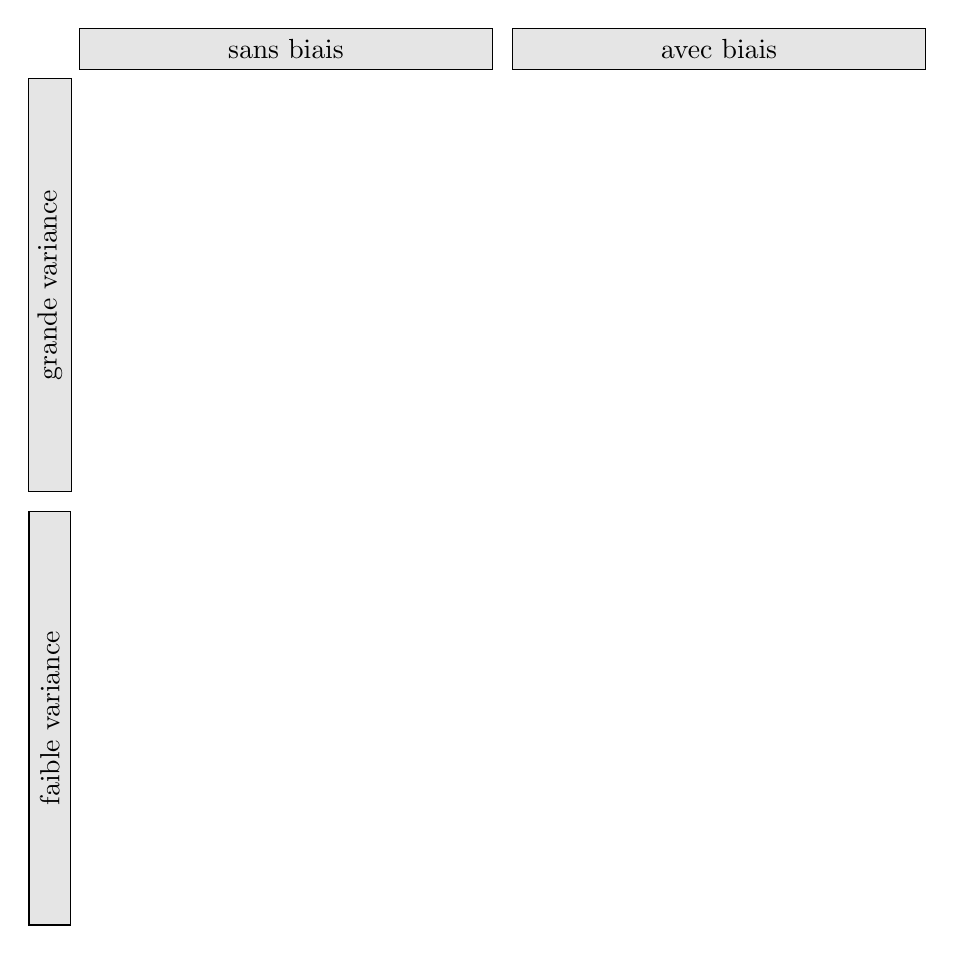
\begin{tikzpicture}[
  labeltext/.style = {
    draw, minimum width = 5.25cm, minimum height = 1.5em, fill = gray!20,
  }]
\pgfmathsetseed{1}%Setting the seed                         
\def\dist{5.5};

\begin{scope}[shift = {(0, 0)}]

  \node[labeltext] at (0, 3) {sans biais};
  \node[labeltext, rotate = 90] at (-3, 0) {grande variance};
  \target

  \points{0}{0}{1}

  \circlevar{0}{0}{1.15}
  \border
\end{scope}

\begin{scope}[shift = {(\dist, 0)}]

  \node[labeltext] at (0, 3) {avec biais};
  \target 

  \points{0.5}{0.50}{1}

  \circlevar{0.5}{0.50}{1.15}
  \border
\end{scope}

\begin{scope}[shift = {(0, -\dist)}]

  \node[labeltext, rotate = 90] at (-3, 0) {faible variance};
  \target

  \points{0}{0}{0.5}

  \circlevar{0}{0}{0.65}
  \border
\end{scope}

\begin{scope}[shift = {(\dist, -\dist)}]

  \target

  \points{0.5}{0.5}{0.5}

  \circlevar{0.5}{0.50}{0.65}
  \border
\end{scope}

\end{tikzpicture}

\end{document}